% Chapter organized by the strength and limits of the geometric evidence.
\section{Finding mathematical patterns with data science}
\label{sec:fresh-data-search}
\label{sec:black-box-datascience}

The normalized sum of symplectic ridge areas is a useful coarse indicator
of systolic ratio, but does not reliably order the bodies selected for
small ridge sums. Its strong inverse association in the broad sample
weakens markedly after restriction to either low ridge sums or high
ratios. Fresh low-ridge selections still have larger mean ratios than
comparison bodies, even where stronger filtering gives no further gain.
The distinction is between identifying a promising population and finding
an improving direction within it.

Affine shape variation of the polygon factors contributes materially to
this pattern. Balancing their vertex covariances raises the mean numerical
ratio from $0.342$ to $0.654$ in a matched sample of 320 products, while
the pooled correlation of within-group ranks weakens from $-0.929$ to $-0.249$.
This supplies a concrete geometric source of variation in the broad
sample. It does not explain all of the remaining association or turn
balancing into a universal improvement rule.

Exact geometry imposes complementary limits on any explanation. Among
polygon products the normalized ridge sum is at least eight, and the cube
attains that minimum with systolic ratio only $1/2$. Minimizing ridge area
therefore cannot maximize the ratio universally. Yet rotated regular
pentagon products satisfy an exact inverse-square relation between the
two quantities. A broader account must accommodate both this strict
family relation and its failure outside that family.

\subsection{The geometric quantities and the sampled populations}
\label{subsec:ds-sampling}

For numerical evaluations we write
$\widehat{\operatorname{sys}}=c_{\mathrm{num}}^2/(2V_{\mathrm{num}})$.
Its normalization agrees with $\operatorname{sys}$; its volume is computed
in floating-point arithmetic. The empirical results below concern this
numerical ratio.

A two-dimensional face of a four-dimensional polytope is called a ridge.
For a ridge $F$ with cyclically ordered vertices $v_0,\ldots,v_{r-1}$, define
its absolute symplectic area by
\[
 A_\omega(F)=\frac12\left|\sum_{i=0}^{r-1}\omega_0(v_i,v_{i+1})\right|,
 \qquad v_r=v_0,\qquad
 \omega_0=dq_1\wedge dp_1+dq_2\wedge dp_2.
\]
This is the polygonal area formula with the symplectic pairing in place of
the planar determinant. It measures the area seen by $\omega_0$; a ridge can
have positive Euclidean area and zero symplectic area. Two summaries proved
useful:
\[
 R(K)=\frac{\sum_F A_\omega(F)}{\sqrt{\operatorname{vol}_4(K)}},
 \qquad
 C(K)=\frac{\max_F A_\omega(F)}{\sum_F A_\omega(F)}.
\]
The first records total symplectic ridge area relative to volume. The second
records the fraction concentrated on the largest ridge, when the total is
positive. Both are unchanged by translation, common dilation and linear
symplectic maps. The area formula is translation invariant because the terms involving the
translation vector cancel around the closed polygon.


The exploratory sample contains 4,096 generic four-dimensional polytopes,
with 512 at each facet count $F=5,\ldots,12$, and 10,240 Lagrangian products
$P\times Q$, with 1,024 at each pair $3\leq k\leq m\leq6$ of factor side
counts. In coordinates $(q_1,q_2,p_1,p_2)$, $P$ lies in the $q$-plane and
$Q$ in the $p$-plane. A fixed facet count or pair of side counts defines a
sample group.

The unit facet normals are independent and uniform on the appropriate
sphere, and the support heights are independent and uniform in
$[0.8,1.2)$. Boundedness and the presence of every proposed facet are
required. Thus these are specified distributions of bodies; the precise
admission rules are in Appendix~\ref{app:ds-generation}. The largest
numerical ratio in the exploratory sample is $0.863$. Its retained values
and current reevaluation are described in Appendix~\ref{app:ds-evaluation}.

\subsection{A strong bulk association weakens under selection}


The pooled rank correlation between $R$ and the numerical systolic ratio is about $-0.94$. Rank correlation compares the orderings of the bodies by the two quantities; a value of $-1$ would mean exactly reversed orderings. The ordinary linear correlation is much weaker, about $-0.21$. Thus the principal observation concerns which bodies have larger systolic ratio, rather than how much the systolic ratio changes per unit of ridge area. The inverse association also occurs within every sampled facet-count or polygon-size group: the rank correlations range from about $-0.84$ to $-1.00$. Thus it is not solely a consequence of pooling these groups. Figures~\ref{fig:ds-ridge-association} and~\ref{fig:ds-ridge-products} show the separate populations.

Conditioning the original sample on either low $R$ or high numerical
systolic ratio weakens this association. If the lowest ten percent by $R$
are retained within each group, the pooled correlation of within-group
ranks is $-0.222$; retaining the highest ten percent by ratio gives
$-0.286$, compared with $-0.944$ before restriction. Figure~\ref{fig:ds-conditional-ranks}
shows the progressive attenuation. At the five-percent cutoff the
high-ratio panel still has a negative association, so attenuation should
not be confused with independence. The smallest panels contain only six
generic or eleven product bodies per group.

\begin{figure}[!htbp]
\centering
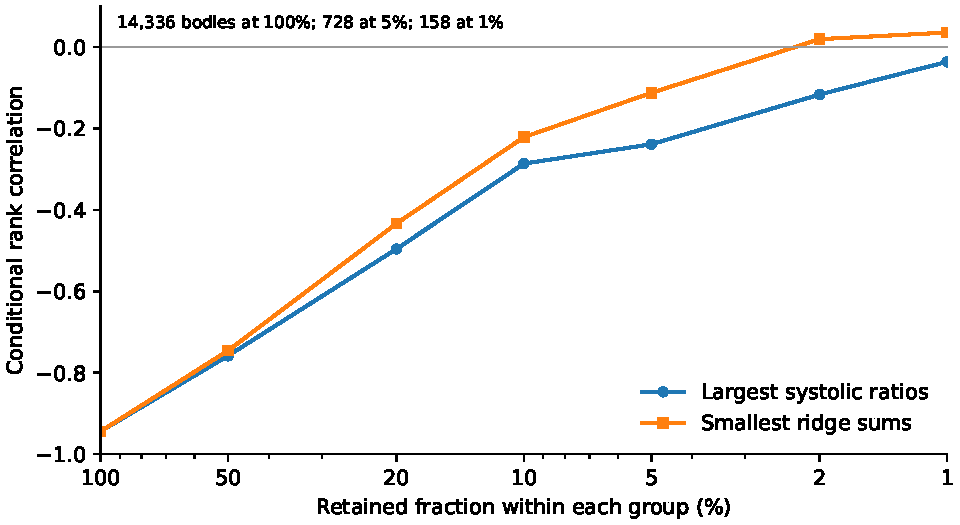
\includegraphics[width=.94\linewidth]{ds-complete-draft/figures/conditional-ridge-correlation.pdf}
\caption{Restricting the original sample by either ridge sum or systolic
ratio weakens their inverse association. Within each facet-count or
factor-side-count group, retain the indicated fraction, rerank both
quantities within that retained group, and compute the pooled Spearman
correlation of the group-relative ranks. This is a descriptive conditional
analysis of the original data. It does not evaluate a fresh selection
rule or identify a geometric cause.}
\label{fig:ds-conditional-ranks}
\end{figure}

The attenuation is substantially stronger than in a Gaussian reference
fitted separately to each group's full-sample rank correlation. At the
five-percent cutoff, that reference gives mean correlation $-0.695$ for
either selection, versus the observed $-0.239$ for high ratios and
$-0.113$ for low $R$. This reference does not reproduce the conditional
pattern; it does not exclude range-restriction effects under other
dependence structures. Its construction is in Appendix~\ref{app:ds-selection}.

Ridge measurements also contain predictive information beyond face counts
and incidences. Under a common training/test split, ridge-area features
alone gave test $R^2=0.887$, whereas combinatorial counts alone gave
$0.043$. Here $R^2$ compares squared prediction error with prediction by
the test-set mean. The feature lists, additional models and split
definitions are in Appendix~\ref{app:ds-prediction}.

\begin{figure}[p]
\centering
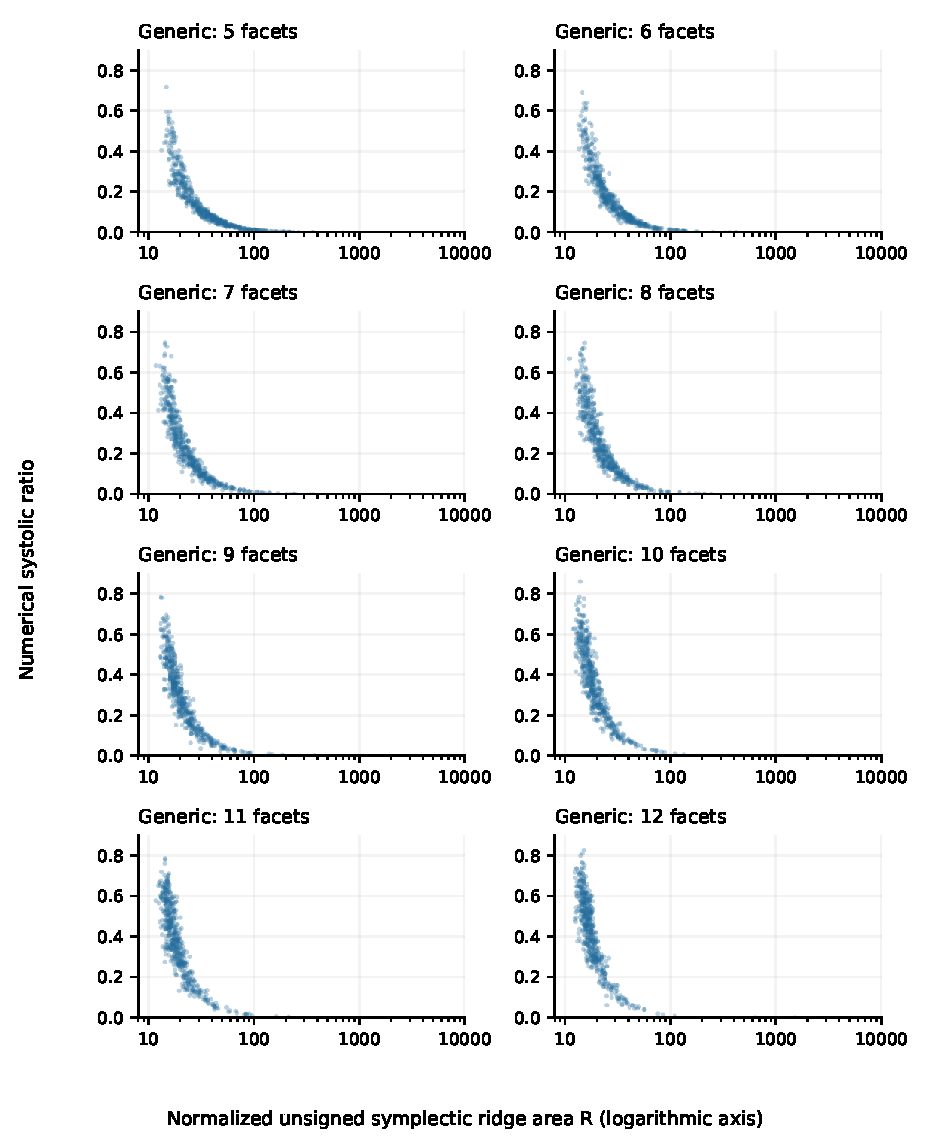
\includegraphics[width=\linewidth]{ds-complete-draft/figures/association-generic.pdf}
\caption{Ridge area and numerical systolic ratio for the 4,096 generic
polytopes, separated by facet count. Each point is one body; the horizontal
axis is logarithmic. All original numerical values are retained
(Appendix~\ref{app:ds-evaluation}).}
\label{fig:ds-ridge-association}
\end{figure}
\begin{figure}[p]
\centering
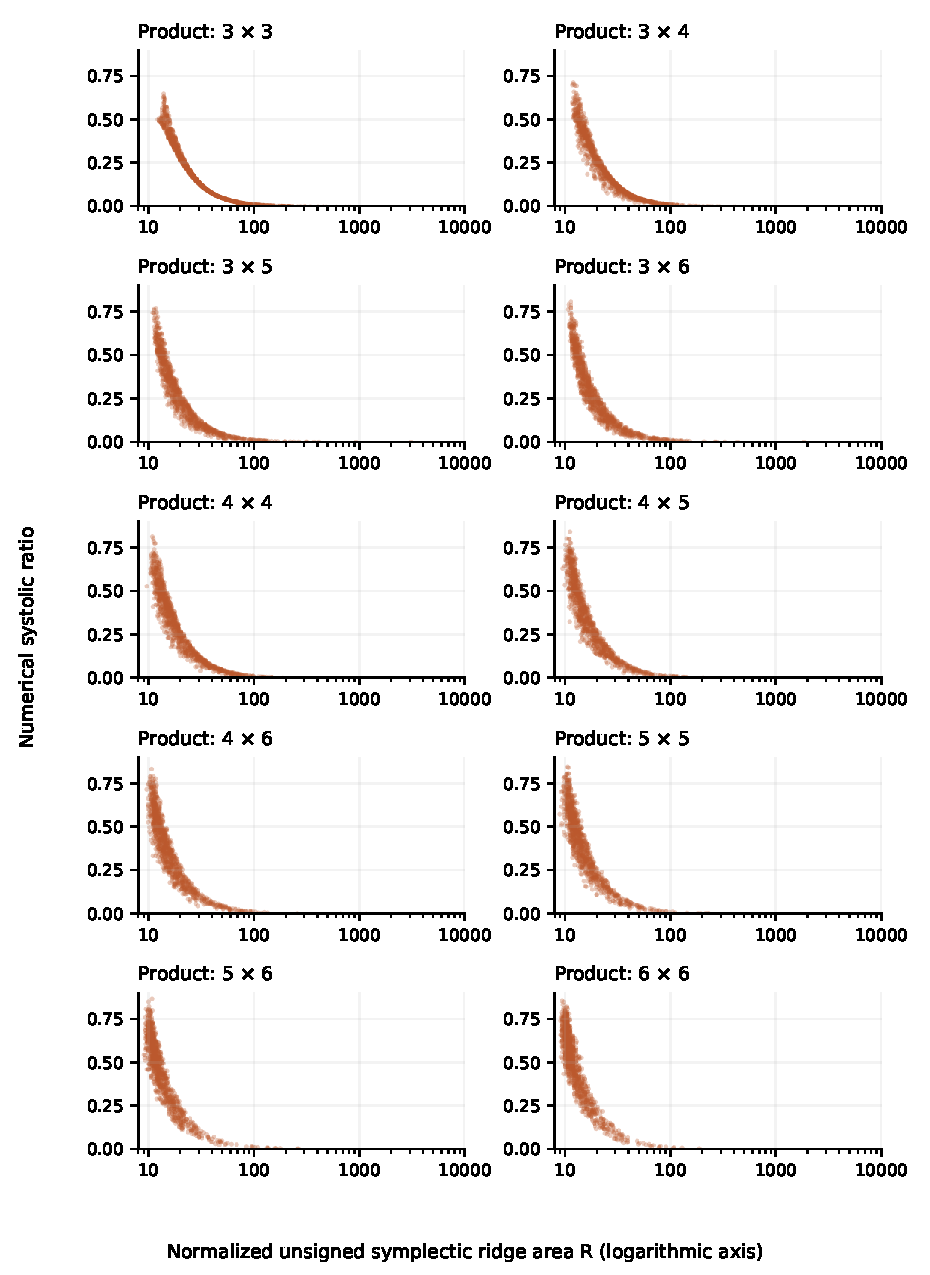
\includegraphics[width=\linewidth]{ds-complete-draft/figures/association-products.pdf}
\caption{The same comparison for the 10,240 Lagrangian products, separated
by factor side counts. Each group contains 1,024 bodies.}
\label{fig:ds-ridge-products}
\end{figure}

\FloatBarrier
\subsection{Exact geometry: a special law and its limits}

A universal inverse relation between ridge sum and systolic ratio is
false, but it can hold exactly on a restricted family. The product edge
formula explains both statements and identifies the smallest possible
ridge sum among polygon products.

For products the descriptor has an elementary edge formula. Let $u_i$ and $v_j$ be
the counterclockwise boundary edge vectors of $P$ and $Q$. A ridge lying entirely in a $q$-
or $p$-plane has zero symplectic area. A mixed ridge is the rectangle formed
from one edge in each factor, and its symplectic area is $|u_i\cdot v_j|$.
Consequently
\[
 R(P\times Q)=\frac{\sum_{i,j}|u_i\cdot v_j|}
                    {\sqrt{\operatorname{area}(P)\operatorname{area}(Q)}}.
\]
For a fixed $u_i$, the sum over the edges of $Q$ is the total variation of
the projection of its boundary onto the direction of $u_i$. Convexity gives
one increasing and one decreasing chain between the extreme projections,
so
\[
 \sum_j|u_i\cdot v_j|
 =2\|u_i\|\,\operatorname{width}_Q(u_i/\|u_i\|).
\]
The descriptor therefore combines the edge lengths of one factor with the
widths of the other in the edge directions. This gives concrete geometry
to investigate instead of treating the successful column as an unexplained
score.


\paragraph{The minimum ridge sum for polygon products.}
Let $P,Q$ be convex polygons with nonempty interior, set $D=P-P$, and write
$A_P,A_Q$ for their areas. Let $J_2(x,y)=(-y,x)$, and normalize mixed area, for $t\geq0$, by
\[
 \operatorname{area}(K+tL)=\operatorname{area}(K)+2tV(K,L)
                         +t^2\operatorname{area}(L).
\]
Then
\begin{equation}\label{eq:ds-product-ridge-minimum}
 R(P\times Q)=\frac{4V(D,J_2Q)}{\sqrt{A_PA_Q}}\geq8.
\end{equation}
Equality holds precisely when $P$ is centrally symmetric and $J_2Q$ is
positively homothetic to $D$, allowing translation.

\begin{proof}
Let $h_D$ be the support function of $D$. The boundary-projection identity
gives $\sum_i|u_i\cdot v_j|=2h_D(v_j)$. The outward unit normal to the
counterclockwise edge $J_2v_j$ is $v_j/\|v_j\|$. The polygon mixed-area
formula therefore gives
\[
 2V(D,J_2Q)=\sum_j\|v_j\|h_D(v_j/\|v_j\|)
          =\sum_j h_D(v_j),
\]
which proves the identity. Brunn--Minkowski and its equality case
\cite[Sections~3 and~5]{dsGardner2002} imply
\[
 V(D,J_2Q)^2\geq\operatorname{area}(D)A_Q,
 \qquad \operatorname{area}(D)\geq4A_P.
\]
The first inequality is an equality exactly when $D$ and $J_2Q$ are
positively homothetic. The second is an equality exactly when $P$ is
centrally symmetric. Substitution proves the bound and equality statement.
\end{proof}

For two aligned unit
squares, eight edge pairs have absolute scalar product one and the rest
zero, so $R=8$. Their product is the unit four-dimensional cube, whose
capacity is one and whose systolic ratio is $1/2$.\footnote{For the centered
unit cube the dual rows are $\pm2e_i$. In the variational formula, closure
forces equal weights $x_j$ on the two $q_j$ rows and equal weights $y_j$ on
the two $p_j$ rows, with $\sum_{j=1}^2(x_j+y_j)=1/2$. The order of the four
rows in a coordinate pair gives a contribution at most $8x_jy_j$ to $Q$.
Thus $Q\leq8\sum_jx_jy_j\leq1/2$. A cyclic word on one coordinate pair
with its four weights equal to $1/4$ attains $Q=1/2$, giving $c=1/(2Q)=1$.} HKO has the larger ridge
score $8.944$ and a ratio greater than one. Thus a universal claim that
a smaller ridge score forces a larger systolic ratio is false. The strong
negative association in the sampled distributions needs a more specific
explanation.


In particular, the cube attains the global minimum of $R$ among polygon
products without attaining a large systolic ratio. The HKO value is also
not separated from ordinary sampled bodies by $R$: its value $8.944$
exceeds the exploratory sample minimum $8.926$.

For rotated regular pentagons, the descriptor does have an exact relation
to capacity. Let $K_\theta=P_5\times\operatorname{Rot}(\theta)P_5$, with circumradius one,
and let $d(\theta)=\min_{k\in\mathbb Z}|\theta-k\pi/5|$.
Each edge has length $2\sin(\pi/5)$ and each factor has area
$5\sin(\pi/5)\cos(\pi/5)$. The mixed-edge formula therefore gives
\[
 R(K_\theta)=4\tan(\pi/5)
       \sum_{k=0}^4|\cos(\theta+2\pi k/5)|
     =16\sin(\pi/5)\cos d(\theta).
\]
For the second equality, the absolute-cosine sum is even and has period
$\pi/5$. On $[-\pi/10,\pi/10]$, the terms indexed by $0,1,4$ are
nonnegative and those indexed by $2,3$ are nonpositive. Pairing opposite
indices reduces the sum to
$[1+2\cos(2\pi/5)-2\cos(4\pi/5)]\cos\theta
=4\cos(\pi/5)\cos\theta$.
Combining this with the capacity profile proved in
Theorem~\ref{thm:rotated-pentagon-product-formula} yields
\begin{equation}\label{eq:ds-pentagon-ridge-capacity}
 \operatorname{sys}(K_\theta)R(K_\theta)^2=16(3+\sqrt5).
\end{equation}
Thus smaller normalized total unsigned ridge area means larger systolic
ratio within this rotation family. This supplies a geometric explanation
for one instance of the observed inverse association.


More precisely, $R$ strictly decreases and $\operatorname{sys}$ strictly
increases as $d$ runs from $0$ to $\pi/10$. Throughout this rotation
family, distinct ridge sums therefore have strictly reversed systolic
ratios. The periodicity and reflection symmetry prevent strict
monotonicity in the unrestricted angle $\theta$.

The exact relation is special to this family. Along sampled rotation
paths of $3\times6$ and $4\times4$ products, both $R$ and the numerical
ratio decrease at the four recorded positions. These observations do not
establish monotonicity between those positions. Together with the exact
cube--HKO comparison, they show why a relationship visible in one family
cannot be extrapolated to every deformation or product.

\subsection{Coarse selection succeeds; stronger selection need not}

The bulk association has a practical consequence: geometry alone can
identify fresh populations with larger numerical ratios before capacity
is evaluated. Within fixed factor-side-count groups, selection for low
$R$ gave mean ratio $0.626$, compared with $0.316$ for comparison bodies
from the same source. Among products already in the lowest one percent
by $R$, the half with lower $C$ had a further mean advantage of $0.034$
over the other half, positive in eight of ten groups. Thus the dominance
of the largest ridge contains information even when the total ridge area
is small. This concerns largest-ridge dominance, rather than every notion
of how evenly area is distributed.

The strong ordering in the broad samples is not retained within the
low-$R$ panels themselves. Across 1,000 evaluated products in the lowest
one percent by $R$, correlations within the ten side-count groups range
from $-0.315$ to $+0.301$; pooling ranks computed within each group gives
$+0.032$. The most extreme tenth has a larger mean ratio than the rest
in only two groups. Coarse enrichment over comparison bodies and loss of
the inverse ordering within the selected population are therefore both
visible in the same research program.

For generic ten-facet bodies, the related score $R/N_2$, where $N_2$ is
the number of ridges, measures normalized area per ridge. Unlike products
at fixed side counts, these bodies can have different ridge counts.
Selecting the lowest one percent by $R/N_2$ gave mean ratio $0.626$,
against $0.339$ for comparison bodies. Within that selected panel, however,
the ten most extreme scores had a mean ratio $0.032$ below the remaining
ninety. This is a failure to obtain further gain in that sample, not an
established deterioration under every stronger filter. The comparison
rules and conditional resampling summaries are retained in
Appendix~\ref{app:ds-selection}.

The area decomposition supplies a geometric view of the same limitation.
For Euclidean ridge area $E(F)>0$, write
\[
 A_\omega(F)=E(F)\kappa(F),\qquad
 \kappa(F)=A_\omega(F)/E(F).
\]
Here $\kappa$ measures the alignment of the ridge plane with the symplectic
form relative to the Euclidean metric. Neither factor is invariant under
all linear symplectic maps. In the generic selection, both mean normalized
Euclidean ridge area and Euclidean-area-weighted $\kappa$ were smaller
than in the comparison panel: $0.917$ versus $1.365$, and $0.377$ versus
$0.503$. Within the selected panel, the ten lowest ridge scores instead
had slightly larger ordinary area and smaller alignment factor than the
other ninety, without a larger mean ratio. Lowering one component is
therefore not enough to explain or guarantee improvement.

\subsection{The inverse direction survives a controlled change of shape}

The attenuation under selection does not mean that the inverse relation
is confined to comparisons of unrelated bodies. Keeping polygon normals
fixed and setting both factors' support heights to one gives opposite
changes in $R$ and the numerical systolic ratio in fifteen of sixteen
pairs. In ten pairs $R$ decreased and the ratio increased; in five the
reverse happened. Both quantities increased in the remaining pair.
Thus the sign relation persists for most of these controlled changes,
even though making the factors tangential does not always raise the ratio.

Separate normalization of the factors preserves the ratio: for $a,b>0$,
\[
 \operatorname{diag}(aI_2,bI_2)
 =\sqrt{ab}\,\operatorname{diag}(\sqrt{a/b}\,I_2,\sqrt{b/a}\,I_2)
\]
is a dilation followed by a symplectic map. Thus replacing unequal support
heights is the geometric change being tested.

The evidence is stronger for direction than for size of effect. The
Spearman correlation between the two changes is $-0.55$ overall and only
$-0.095$ in the $4\times6$ group. All tested ratios are at most $0.742$,
so this is not a deformation test of the high-ratio tail. It is consistent
with shared geometric variation producing the bulk association, but does
not isolate a causal role for ridge area or explain the whole pattern.
The paired constructions and checks are in
Appendix~\ref{app:ds-deformations}.

\subsection{Covariance balance gives a second geometric signal}

Ridge area is not the only summary associated with the ratio. In an
exploratory analysis, more nearly equal symplectic covariance scales of
the vertex set were associated with larger ratios. For vertices
$v_1,\ldots,v_N$, define
\[
 \overline v=\frac1N\sum_i v_i,\qquad
 \Gamma=\frac1N\sum_i(v_i-\overline v)(v_i-\overline v)^T.
\]
In Williamson normal form, $\Gamma$ has diagonal
$(\nu_1,\nu_2,\nu_1,\nu_2)$, with $0<\nu_1\leq\nu_2$.
The ratio $\rho=\nu_2/\nu_1$ measures the imbalance between the two
symplectic covariance scales.

Like $R$, this score is invariant under affine symplectic maps and common
dilation. Centering removes translations. For symplectic $S$,
$\Gamma(SK)=S\Gamma(K)S^T$, so with
$J=\left(\begin{smallmatrix}0&I_2\\-I_2&0\end{smallmatrix}\right)$,
\[
 J\Gamma(SK)=S^{-T}(J\Gamma(K))S^T.
\]
The eigenvalues $\pm i\nu_1,\pm i\nu_2$ are unchanged. Dilation multiplies
both $\nu_j$ by the same square factor. For a product with planar vertex
covariances $A,B$, moreover, $\Gamma=\operatorname{diag}(A,B)$ and
$(J\Gamma)^2=\operatorname{diag}(-BA,-AB)$; thus $\nu_1^2,\nu_2^2$ are
the eigenvalues of $AB$.

Low $\rho$ selected larger mean ratios in every side-count group in each
of two fresh pools. The twenty gains over comparison bodies ranged from
$0.260$ to $0.440$, with mean $0.333$. Against the combined low-$R$,
low-$C$ selector, its mean advantage was only $0.014$, and the differences
changed sign across groups. Both geometric summaries therefore support
selection in the tested populations; neither was uniformly better there.

Their usefulness also survived one change of sampling law. For tangential
factors obtained by setting the support heights to one, the mean gains
were $0.259$ for covariance selection and $0.225$ for ridge selection,
averaged equally over the $4\times6$ and $6\times6$ groups. This is one
conditioned source, requiring both original and changed polygons to be
valid. It establishes a particular transfer, not independence from the
sampling distribution. Details are in Appendix~\ref{app:ds-selection}.

\subsection{Balancing the factors improves most tested products}

Removing the planar vertex-covariance anisotropy of both factors raises
the mean numerical ratio from $0.342$ to $0.654$ in a matched comparison
of 320 products, with increases in 314 and decreases in six. At the same
time, the pooled within-group rank correlation between $R$ and the ratio
weakens from $-0.929$ to $-0.249$. Thus affine shape variation of the
factors contributes materially to the broad association in this sample.

The transformation has a precise geometric meaning. For a factor with
vertex covariance $A$, set
\[
 L_A=(\det A)^{1/4}A^{-1/2}.
\]
Then $\det L_A=1$ and
$L_A A L_A^T=\sqrt{\det A}\,I_2$. Applying $L_A$ and $L_B$ to the two
factors preserves their areas and combinatorics and makes both vertex
covariances scalar matrices. The product therefore has $\rho=1$.
These independent factor maps need not combine to a symplectic map, so
capacity can change even though volume is preserved.

The mean ridge sum falls from $23.739$ to $11.652$, decreasing in 306 of
the 320 products. The remaining relation depends on the side counts:
the balanced $3\times3$ group has positive rank correlation, while the
other nine groups retain negative correlations. The transformation changes
several geometric properties together. It therefore identifies a useful
shape deformation, not covariance imbalance as the sole cause of the
bulk association. Nor do its six decreases permit a universal improvement
rule. The target-blind choice of original bodies, complete paired
evaluations and numerical checks are in Appendix~\ref{app:ds-balance}.

\subsection{What could explain the bulk association?}

The controlled changes give substance to one possible explanation of the
bulk pattern. Many original products leave a large improvement available
under factor balancing, and removing that shape variation weakens the
association. Common perturbations of relatively inefficient shapes could
therefore account for much of the broad inverse ordering, while other
features govern differences among the better bodies. The height changes
supply a second concrete deformation with a mostly inverse direction.
Neither experiment measures geometric distance to a local optimum or
establishes an additive-noise model.

A different explanation is an underlying relation involving a geometric
quantity that $R$ measures only imperfectly. Extreme $R$ can then reflect
both favorable geometry and deviations specific to the proxy. Here noise
would mean differences between bodies not captured by the relation, not
numerical error in a fixed-body evaluation. The residual associations
after balancing leave room for such a relation; they do not identify it.

These explanations are compatible, and the results do not choose between
them. The observed attenuation is stronger than in the fitted Gaussian
reference, but other dependence structures can behave differently under
selection. Neither convenient account need describe the full phenomenon.
The exact pentagon identity, the global counterexample and the controlled
shape changes provide constraints that a broader explanation must respect.

\subsection{Using evaluated ratios to guide search}

A weak explanation of the ridge signal need not prevent practical search.
Adapting the product sampling law to evaluated ratios improved both the
maximum and the quality of several leading bodies in three paired runs.
For $5\times5$ products, the cross-entropy method~\cite{dsDeBoer2005}
shifts a fitted distribution towards the quarter of the current population
with largest ratios, then samples again. Under equal evaluation counts,
the results were:
\begin{center}
\begin{tabular}{crrrr}
\hline
 & \multicolumn{2}{c}{Maximum} & \multicolumn{2}{c}{Top-eight median}\\
Seed & IID & Adaptive & IID & Adaptive\\
\hline
1 & .760 & .799 & .729 & .782\\
2 & .811 & .831 & .754 & .776\\
3 & .760 & .856 & .722 & .814\\
\hline
\end{tabular}
\end{center}
The top-eight statistic is the median of the eight highest ratios after
removing repeated exact dual-vertex arrays. Both arms share their initial
population. The fitted coordinates describe log ratios of normal-angle
gaps, centered logarithmic dual-normal lengths and a relative angle;
the latter uses a circular mean update. The coordinate-dependent evaluator
admission condition acts differently on the original sampling coordinates
and the adaptive normalized representation. The observed advantage
therefore concerns this implemented combination of adaptation and
admission. Appendix~\ref{app:ds-adaptive} records the update, budgets and
admission history.

The prescribed ambient rotations $K\mapsto UK$, $U\in SO(4)$, also
lost to fresh sampling under equal evaluation budgets. These limited
comparisons are recorded in Appendix~\ref{app:ds-deformations}.

\subsection{Competing branches in local search}
\label{subsec:black-box-datascience-finite-budget-optimization}

The local-search comparison favors methods that account for several
competing branches of the capacity calculation. A single selected branch
can point uphill while the minimum of the branches decreases. For example,
$\min\{x,-x\}$ decreases in either direction from zero although each
individual branch has an increasing direction. The corresponding search
question is whether retaining nearby or previously active branches helps
the numerical systolic ratio increase.

Seven fixed implementations started from the same 64 generic ten-facet
bodies, under a common cap of 128 full evaluations and a nominal one-second
accumulated evaluator-plus-optimizer budget. The implementations retaining
branches from earlier points attained the largest median terminal values:
\begin{center}
\begin{tabular}{lrr}
\hline
Implementation & Median best value & Across-start $10$--$90\%$ range\\
\hline
Four-anchor history & .985 & .957--.999\\
History with transition prediction & .982 & .956--.994\\
Finite-gap model & .977 & .948--.995\\
Literal gradient & .881 & .790--.924\\
Safeguarded gradient & .855 & .780--.916\\
CMA-ES & .818 & .718--.869\\
Coordinate poll & .601 & .358--.787\\
\hline
\end{tabular}
\end{center}
The finite-gap method models branches near the current minimum. The two
history methods also retain earlier branches; one predicts additional
branches from transitions. CMA-ES~\cite{dsHansen2016} and coordinate polling
supply population and direct-search comparisons. These are rankings of
the fixed implementations under this allocation, not of optimally tuned
algorithm families. The historical numerical objective uses floating-point
geometry and volume, and not every original executable or proposal trace
was recovered. Appendix~\ref{app:datascience-results} gives the retained
steps, provenance and budget interpretation. The ranges in the table
show variation across starting bodies; all 448 terminal values are below one.

\subsection{A failed probe does not establish a local maximum}

The endpoint diagnostics show that a high terminal ratio need not mean
local convergence. One optimizer endpoint decreased along every tested
signed basis direction, yet a continuation increased its ratio by
$0.00223$ along oblique moves of total normalized path length $0.01$.
All three selected endpoints in that continuation accepted ten improving
steps, while HKO accepted none. HKO's local status is established by its
theorem; the finite test supplies a consistent control observation.

A regular-pentagon control on a known increasing rotation path illustrates
the same problem independently. In a suite of basis, random and prescribed
rotation probes, its only positive changes were the twelve rotation
probes; the generic directions missed the available increase. The regular
triangle--hexagon product, rotated square--square product and CH2021
example had no nominal gain above $10^{-12}$ in that suite. Their misses
do not exclude untested directions or changes in facet count. The probe
design and numerical limitations are in Appendix~\ref{app:ds-probes}.

The chapter therefore supports a strong coarse association, an exact law
on one rotation family, and useful finite search improvements. It does
not supply a universal capacity law or a general route to local optimality.
None of the random samples or search comparisons produced a numerical
ratio above one. For products with a triangle or quadrilateral factor,
the Viterbo inequality is already known~\cite[Theorem~1.2 and Section~4]{dsBMP2026};
such products can illuminate the pattern but cannot yield counterexamples
while remaining in that class. The remaining product families and generic
polytopes leave open both questions: what geometric relation explains the
signal, and what search directions remain effective near large ratios?
